\documentclass[preview]{standalone}

\usepackage{amsmath}
\usepackage{amssymb}
\usepackage{stellar}
\usepackage{definitions}
\usepackage{bettelini}
\usepackage{tikz}

\begin{document}

\id{graph-planar-graphs}
\genpage

\section{Planar graphs}

\begin{snippetdefinition}{planar-graph-definition}{Planar graph}
    A finite \graph \(G\) is \emph{planar} if it can be represented in the
    plane in such a way that:
    \begin{itemize}
        \item vertices are represented by points of the plane;
        \item edges are represented by arcs joining the points corresponding
        to their endpoints;
        \item two arcs do not intersect except possibly at common endpoints.
    \end{itemize}
\end{snippetdefinition}

\begin{snippet}{planar-graph-arc-explanation}
    In the definition of a planar graph, an \emph{arc} means a continuous
    curve representing a topological segment in the plane. For loops, the
    initial point and final point of the arc are allowed to coincide.
\end{snippet}

\begin{snippetexample}{planar-graph-example}{A planar graph}
    The following graph is planar:
    \[
        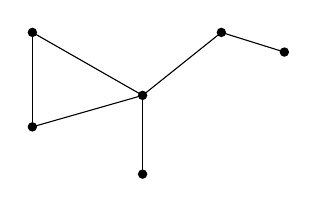
\begin{tikzpicture}[scale=1]
            \coordinate (a) at (0,0);
            \coordinate (b) at (0,1.2);
            \coordinate (c) at (1.4,0.4);
            \coordinate (d) at (1.4,-0.6);
            \coordinate (e) at (2.4,1.2);
            \coordinate (f) at (3.2,0.95);

            \draw (a)--(b);
            \draw (b)--(c);
            \draw (a)--(c);
            \draw (c)--(d);
            \draw (c)--(e);
            \draw (e)--(f);

            \foreach \p in {a,b,c,d,e,f}{
                \fill (\p) circle (1.7pt);
            }
        \end{tikzpicture}
    \]
\end{snippetexample}

\begin{snippet}{planar-drawing-warning}
    One must distinguish an abstract graph from one of its drawings in the
    plane. A planar graph may also be drawn in a non-planar way, with crossings
    between edges. The presence of crossings in a particular drawing does not
    prove that the graph is non-planar.
\end{snippet}

\begin{snippetexample}{planar-drawing-of-k4-example}{A planar drawing of a graph with crossings}
    The complete graph \(K_4\) can be drawn with crossings, but it is planar:
    \[
        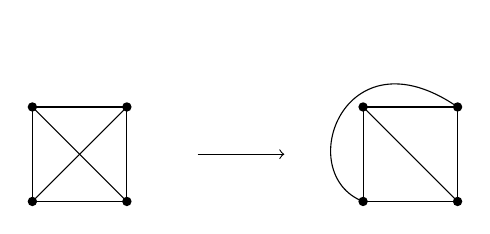
\begin{tikzpicture}[scale=1]
            \begin{scope}
                \coordinate (a) at (0,0);
                \coordinate (b) at (1.2,0);
                \coordinate (c) at (1.2,1.2);
                \coordinate (d) at (0,1.2);

                \draw (a)--(b)--(c)--(d)--cycle;
                \draw (a)--(c);
                \draw (b)--(d);

                \foreach \p in {a,b,c,d}{
                    \fill (\p) circle (1.7pt);
                }
            \end{scope}

            \draw[->] (2.1,0.6)--(3.2,0.6);

            \begin{scope}[xshift=4.2cm]
                \coordinate (a) at (0,0);
                \coordinate (b) at (1.2,0);
                \coordinate (c) at (1.2,1.2);
                \coordinate (d) at (0,1.2);

                \draw (a)--(b)--(c)--(d)--cycle;
                \draw (d)--(b);
                \draw (a) .. controls +(-0.90,0.35) and +(-1.45,1.00) .. (c);

                \foreach \p in {a,b,c,d}{
                    \fill (\p) circle (1.7pt);
                }
            \end{scope}
        \end{tikzpicture}
    \]
\end{snippetexample}

\begin{snippetdefinition}{planar-face-definition}{Face}
    Let \(G\) be a planar \graph together with a fixed planar representation.
    The \emph{faces} of the representation are the connected regions into
    which the representation divides the plane. The unbounded region is also
    counted as a face and is called the \emph{outer face}.
\end{snippetdefinition}

\begin{snippetexample}{planar-faces-example}{Faces of a planar representation}
    The following planar graph has \(4\) vertices, \(6\) edges, and \(4\)
    faces:
    \[
        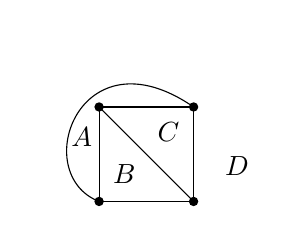
\begin{tikzpicture}[scale=1]
            \coordinate (a) at (0,0);
            \coordinate (b) at (1.2,0);
            \coordinate (c) at (1.2,1.2);
            \coordinate (d) at (0,1.2);

            \draw (a)--(b)--(c)--(d)--cycle;
            \draw (d)--(b);
            \draw (a) .. controls +(-0.90,0.35) and +(-1.45,1.00) .. (c);

            \node at (-0.22,0.82) {\(A\)};
            \node at (0.32,0.35) {\(B\)};
            \node at (0.88,0.88) {\(C\)};
            \node at (1.75,0.45) {\(D\)};

            \foreach \p in {a,b,c,d}{
                \fill (\p) circle (1.7pt);
            }
        \end{tikzpicture}
    \]
\end{snippetexample}

\begin{snippettheorem}{euler-formula-planar-graphs}{Euler's formula for connected planar graphs}
    Let \(G\) be a finite connected planar \graph with a fixed planar
    representation. Let
    \[
        v=\cardinality{V(G)},
        \qquad
        e=\cardinality{E(G)},
        \qquad
        f=\text{number of faces}.
    \]
    Then,
    \[
        v-e+f=2.
    \]
\end{snippettheorem}

\begin{snippetproof}{euler-formula-planar-graphs-proof}{euler-formula-planar-graphs}{Euler's formula for connected planar graphs}
    We show that the quantity
    \[
        v-e+f
    \]
    is invariant under deleting suitable edges that lie on cycles, until a tree
    is obtained.

    If \(G\) is a tree, then it has \(e=v-1\) edges. Moreover, a planar
    representation of a tree encloses no bounded region, so it has only the
    outer face:
    \[
        f=1.
    \]
    Hence
    \[
        v-e+f=v-(v-1)+1=2.
    \]

    Suppose now that \(G\) is not a tree. Since \(G\) is connected, it contains
    at least one cycle. Choose an edge \(a\) lying on a cycle and delete it.
    The resulting graph remains connected, because the endpoints of \(a\) are
    still joined by the rest of the cycle.

    The number of vertices is unchanged, the number of edges decreases by
    \(1\), and the number of faces decreases by \(1\): deleting an edge on a
    cycle merges two adjacent faces into one. Therefore
    \[
        v-(e-1)+(f-1)=v-e+f.
    \]
    Repeating this process finitely many times gives a tree. Since the
    quantity is \(2\) for the final tree, it was already \(2\) for the original
    graph.
\end{snippetproof}

\end{document}
